\documentclass[final]{beamer} % beamer 3.10: do NOT use option hyperref={pdfpagelabels=false} !
% Began with this: https://tex.stackexchange.com/a/24266

\mode<presentation> {  %% check http://www-i6.informatik.rwth-aachen.de/~dreuw/latexbeamerposter.php for examples
  \usetheme{Berlin}    %% you should define your own theme e.g. for big headlines using your own logos 
%  \usetheme{metropolis}

}

\usepackage[english]{babel}
\usepackage[latin1]{inputenc}
\usepackage{amsmath,amsthm, amssymb, latexsym}
\usefonttheme[onlymath]{serif}
\boldmath
\usepackage[size=custom,width=116,height=106.5,scale=3]{beamerposter} % e.g. for custom size poster
\usepackage{graphicx}
%\usepackage{wrapfig}
\usepackage{lmodern}       

\definecolor{forest_green}{RGB}{34,139,34}
\definecolor{usda_green}{RGB}{0,89,65}
\definecolor{dark_magenta}{RGB}{139,0,139}
\definecolor{peru}{RGB}{205,133,63}


%\setbeamercolor{title}{fg=forest_green}
%\setbeamercolor{frametitle}{fg=forest_green}
%\setbeamercolor{structure}{fg=forest_green}
%\setbeamercolor{structure}{fg=usda_green}
%\setbeamercolor{structure}{fg=dark_magenta}
\setbeamercolor{structure}{fg=peru}

\title[Detecting CNV with vcfR]{Copy number variation appears increased in clonal lineages over sexual lineages of \protect\emph{Phytophthora infestans}}
\author[Knaus et al.]{Brian J. Knaus$^{1}$, Javier F. Tabima$^{2}$, Shankar K. Shakya$^{2}$,\\ Howard S. Judelson$^{3}$, and Niklaus J. Gr\"unwald$^{1}$}
\institute[USDA, ARS]{$^{1}$USDA, ARS, Horticultural Crops Research Unit; $^{2}$Oregon State University;\\$^{3}$University of California Riverside}
\date{July 29th, 2018}

\setbeamertemplate{headline}{  
  \leavevmode

  \begin{beamercolorbox}[wd=\paperwidth]{headline}
    \begin{columns}[T]
      \begin{column}{.02\paperwidth}
      \end{column}
      \begin{column}{.7\paperwidth}
        \vskip8ex
        \raggedleft
        \usebeamercolor{title in headline}{\color{fg}\textbf{\large{\inserttitle}}\\[1ex]}
        \usebeamercolor{author in headline}{\color{fg}\normalsize{\insertauthor}\\[1ex]}
        \usebeamercolor{institute in headline}{\color{fg}\small{\insertinstitute}\\[1ex]}     
      \end{column}
      \begin{column}{.15\paperwidth}
        \vskip8ex
        \begin{center}
          
\includegraphics[height=8cm]{./figures/usda-symbol.pdf}\\
          \vspace{3mm}
          
\includegraphics[height=4cm]{./figures/osu_logo.pdf}\\
          \vspace{3mm}
          
\includegraphics[height=2.5cm]{./figures/ucr_logo_cmyk.pdf}
          %Logo goes here.
        \end{center}
        \vskip2ex
      \end{column}
      \begin{column}{.02\paperwidth}
      \end{column}
    \end{columns}
    \vskip2ex
  \end{beamercolorbox}

  \begin{beamercolorbox}[wd=\paperwidth]{lower separation line head}
    \rule{0pt}{0pt}
  \end{beamercolorbox}
}
\setbeamertemplate{footline}{
  \begin{beamercolorbox}[wd=\paperwidth]{upper separation line foot}
    \rule{0pt}{3pt}
  \end{beamercolorbox}

  \leavevmode%
  \begin{beamercolorbox}[ht=4ex,leftskip=1em,rightskip=1em]{author in head/foot}%
    \texttt{http://grunwaldlab.cgrb.oregonstate.edu}
    \hfill
    \texttt{Knaus et al.: CNV in \textit{P. infestans}}
    \vskip1ex
  \end{beamercolorbox}
  \vskip0pt%
  \begin{beamercolorbox}[wd=\paperwidth]{lower separation line foot}
    \rule{0pt}{3pt}
  \end{beamercolorbox}
}

\setbeamertemplate{navigation symbols}{}

\begin{document}
  \begin{frame}{}


    %%%%% %%%%% %%%%%
    %               %
    % New row       %
    %               %
    %%%%% %%%%% %%%%%
\begin{columns}[t]
  \begin{column}{0.44\textwidth}
    \begin{block}{\large Rationale}
%\small
\scriptsize
%\tiny
Inference of copy number variation presents a technical challenge because variant callers typically require the copy number of a genome or genomic region to be known a priori.
Our project required us to address this question, so we designed and implemented a method with the following:

\begin{itemize}
\item No a priori known base ploidy is required
\item Allows for genomic windows to be analyzed
\item Flexibility to use with non-model organisms
\item Works with VCF format data
\item Implemented in R
\end{itemize}

We validated these approaches with the model system of \textit{Saccharomyces cerevisiae}, an organism known to vary in ploidy and copy number.
This method has been implemented in the R package vcfR.
\vspace{3mm}
    \end{block}
  \end{column}

  \begin{column}{0.5\textwidth}
    \begin{block}{\large Chromosomal perspectives}
      \begin{columns}
        \begin{column}{0.4\textwidth}
%\small
%\footnotesize
\scriptsize
%\tiny
\\
\vspace{1mm}
%Different data types provide different perspectives.
Sequence depth can be used to characterize base ploidy and deviations from base ploidy.
However, if a research question includes 'what is base ploidy' we need another perspective.
Allele balance can help provide inferences on whether base ploidy is diploid, triploid, or tetraploid.
This is a reproduction of Figure 7 from Zhou et al. (2016) created in vcfR and highlights chromosome XII as having three copies while base ploidy is two copies.
%\vspace{2mm}
%          \begin{figure}
        \end{column}
        \begin{column}{0.55\textwidth}
          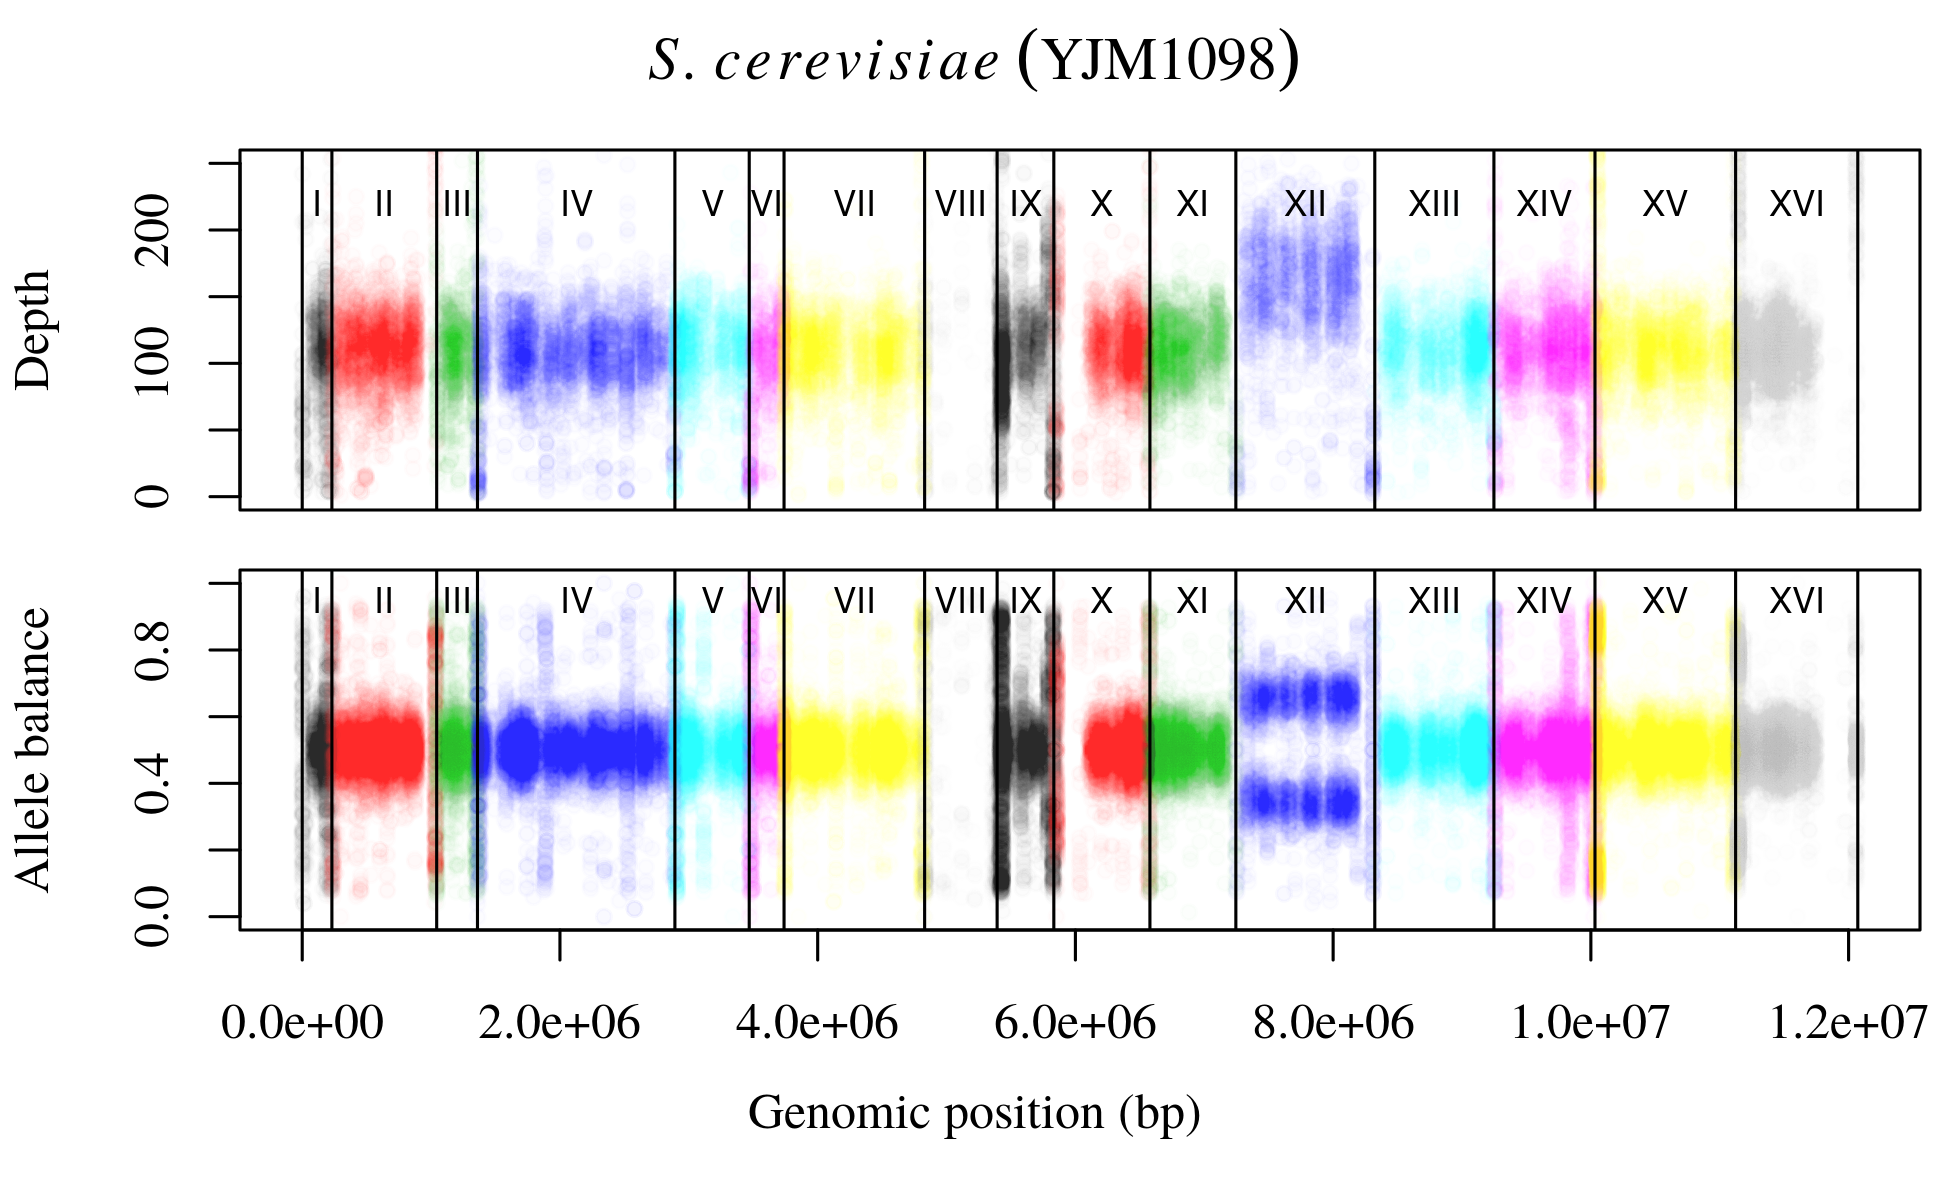
\includegraphics[height=20cm]{./figures/fig4_chrom_YJM1098.png}
        \end{column}
      \end{columns}
%          \caption{Allele balance is the frequency theat the most abundant and second most abundant allele were sequenced at.}
%          \end{figure}

    \end{block}
  \end{column}

\end{columns}




\vspace{5mm}


    %%%%% %%%%% %%%%%
    %               %
    % New row       %
    %               %
    %%%%% %%%%% %%%%%
\begin{columns}[t]
  \begin{column}{0.54\textwidth}
    \begin{block}{\large Copy number does not vary by gene category}
%\small

      \begin{columns}
        \begin{column}{0.5\textwidth}
%\footnotesize
\scriptsize
\vspace{5mm}

Isolates from Mexico typically having two copies of each gene also tended to have two copies of each gene within several annotation categories.
Isolates from South America and US-1 typically had three copies of each gene and also tended to have three copies of each gene within annotation categories.
This indicated that CNV does not prefer particular gene classes.
%          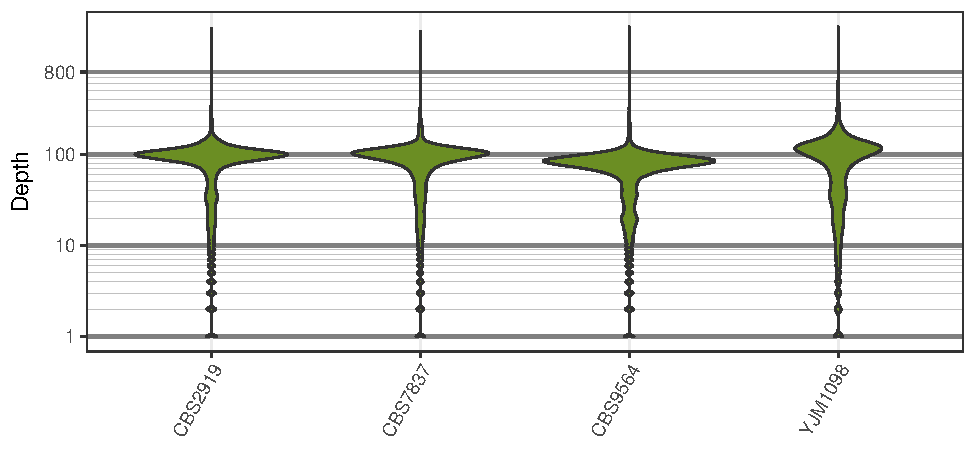
\includegraphics[height=8cm]{./figures/fig2_scer_dp_vplot.pdf}
%          \newline
%          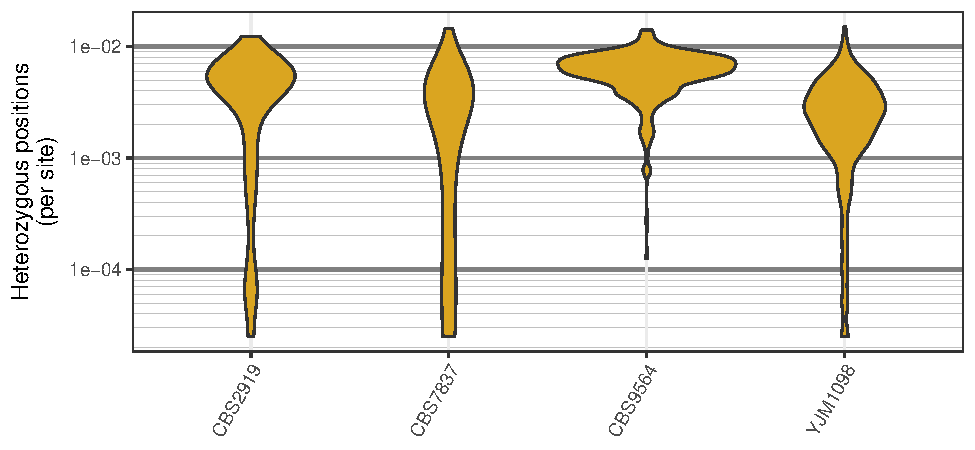
\includegraphics[height=8cm]{./figures/fig3_scer_het_vplot.pdf}
        \end{column}
        \begin{column}{0.45\textwidth}

          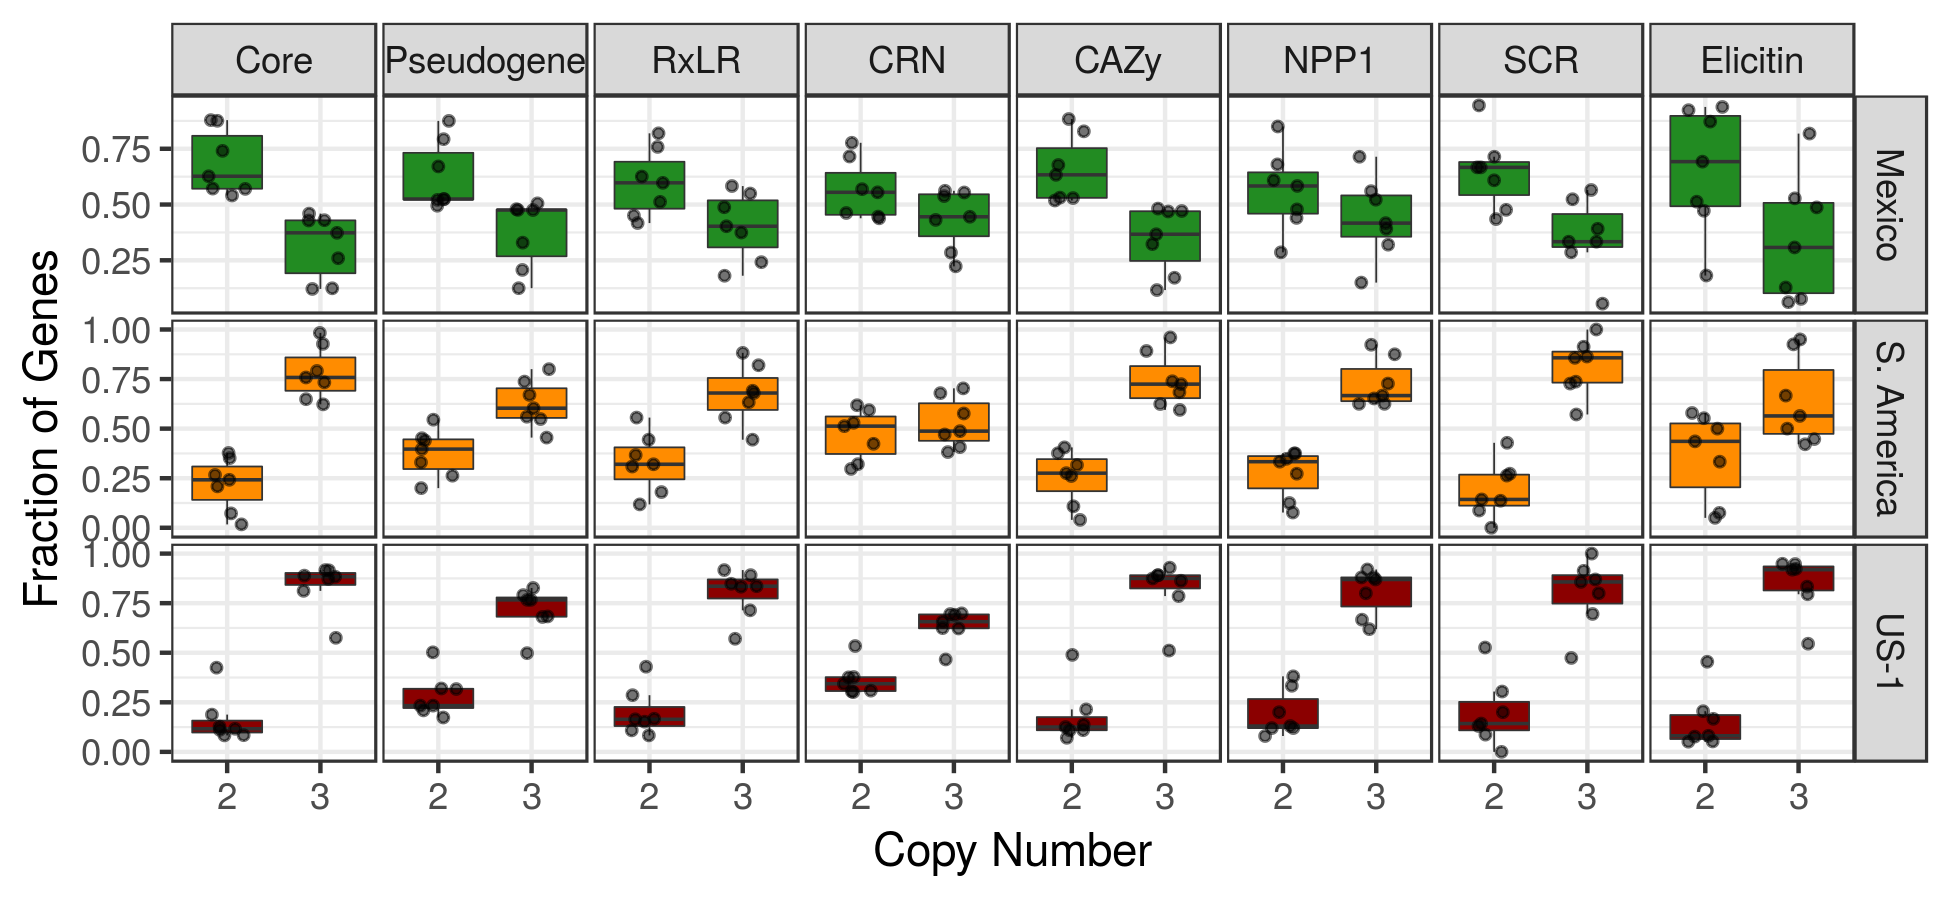
\includegraphics[height=13cm]{./figures/Fig5_gene_cnv.png}

        \end{column}
      \end{columns}

    \end{block}
  \end{column}


  \begin{column}{0.40\textwidth}
    \begin{block}{\large CNV occurs in other species}
      \begin{columns}
        \begin{column}{0.40\textwidth}

          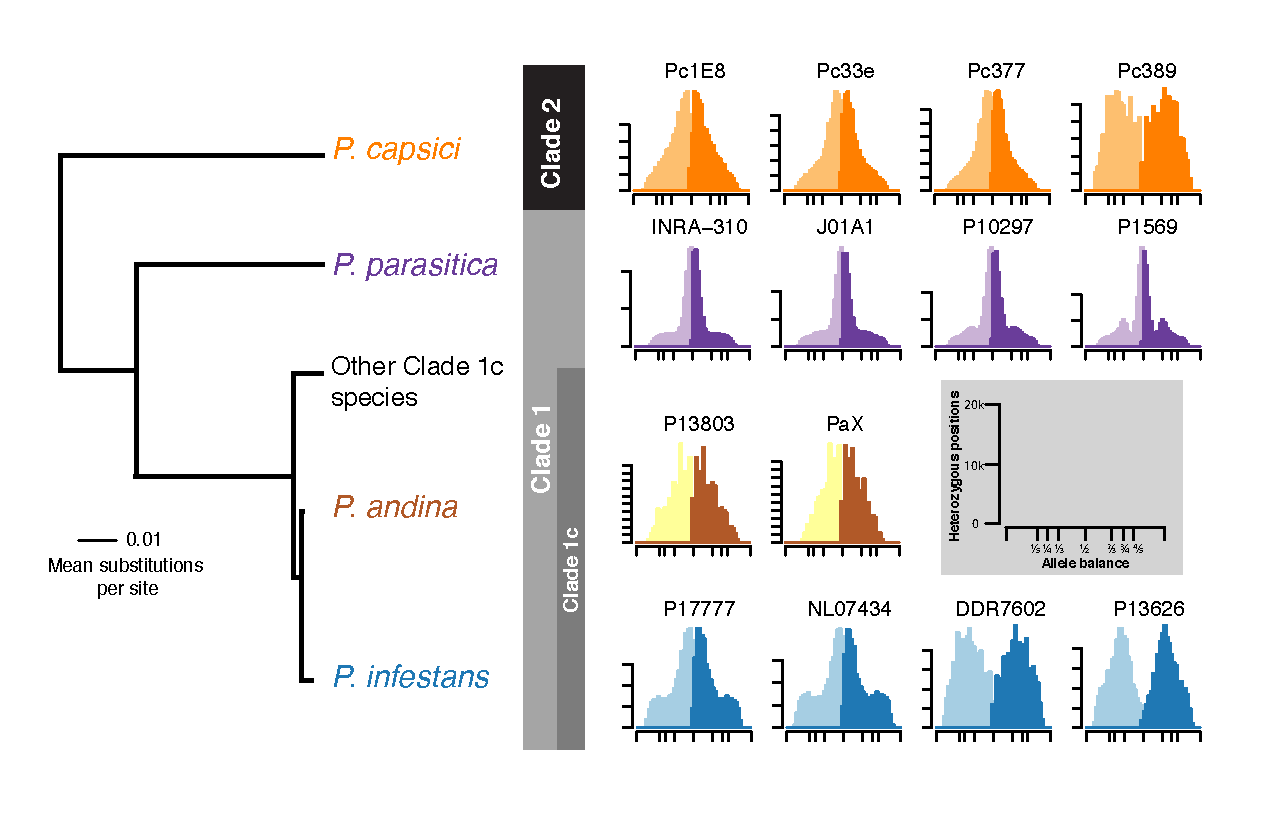
\includegraphics[height=13cm]{./figures/Fig7_ploidy.pdf}

%          \begin{figure}
        \end{column}
        \begin{column}{0.56\textwidth}
%\small
%\footnotesize
\scriptsize
%\tiny
%We used allele balance to explore CNV in other \textit{Phytophthora} genomes that were available at the SRA.
\vspace{5mm}

\textit{P. andina} and \textit{P. parasitica} appeared predominantly diploid.
\textit{P. parasitica} included minor peaks at the expectation for three copies.
Three out of the four \textit{P. capsici} samples appeared predominantly diploid but one appeared triploid.
This indicates that CNV occurs throughout \textit{Phytophthora}.
%          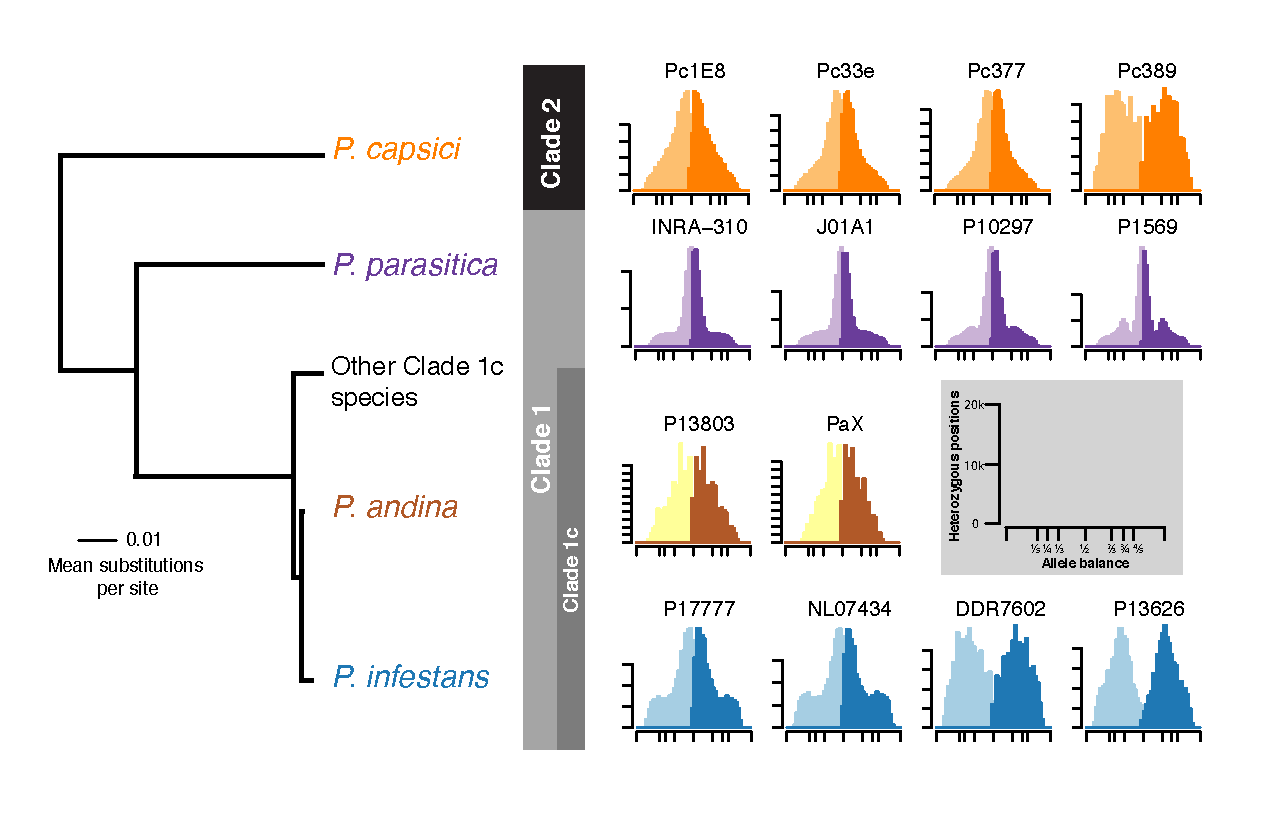
\includegraphics[height=14cm]{./figures/Fig7_ploidy.pdf}
        \end{column}
      \end{columns}
%          \caption{Allele balance is the frequency theat the most abundant and second most abundant allele were sequenced at.}
%          \end{figure}

    \end{block}
  \end{column}


\end{columns}




\vspace{5mm}


    %%%%% %%%%% %%%%%
    %               %
    % New row       %
    %               %
    %%%%% %%%%% %%%%%
\begin{columns}[t]
  \begin{column}{0.65\textwidth}
    \begin{block}{\large Windowing}
      \begin{columns}
        \begin{column}{0.68\textwidth}
%\small
\footnotesize
%\tiny
Allele balance can also be used to assign copy number to genomic windows of variants.
Windows of user specified lengths can be made and allele balance is estimated for each window.
A distance from expectation and the number of heterozygous position for each window are reported to help determine the quality of estimates.
Estimates determined to be of low quality may be censored.
        \end{column}
        \begin{column}{0.30\textwidth}
          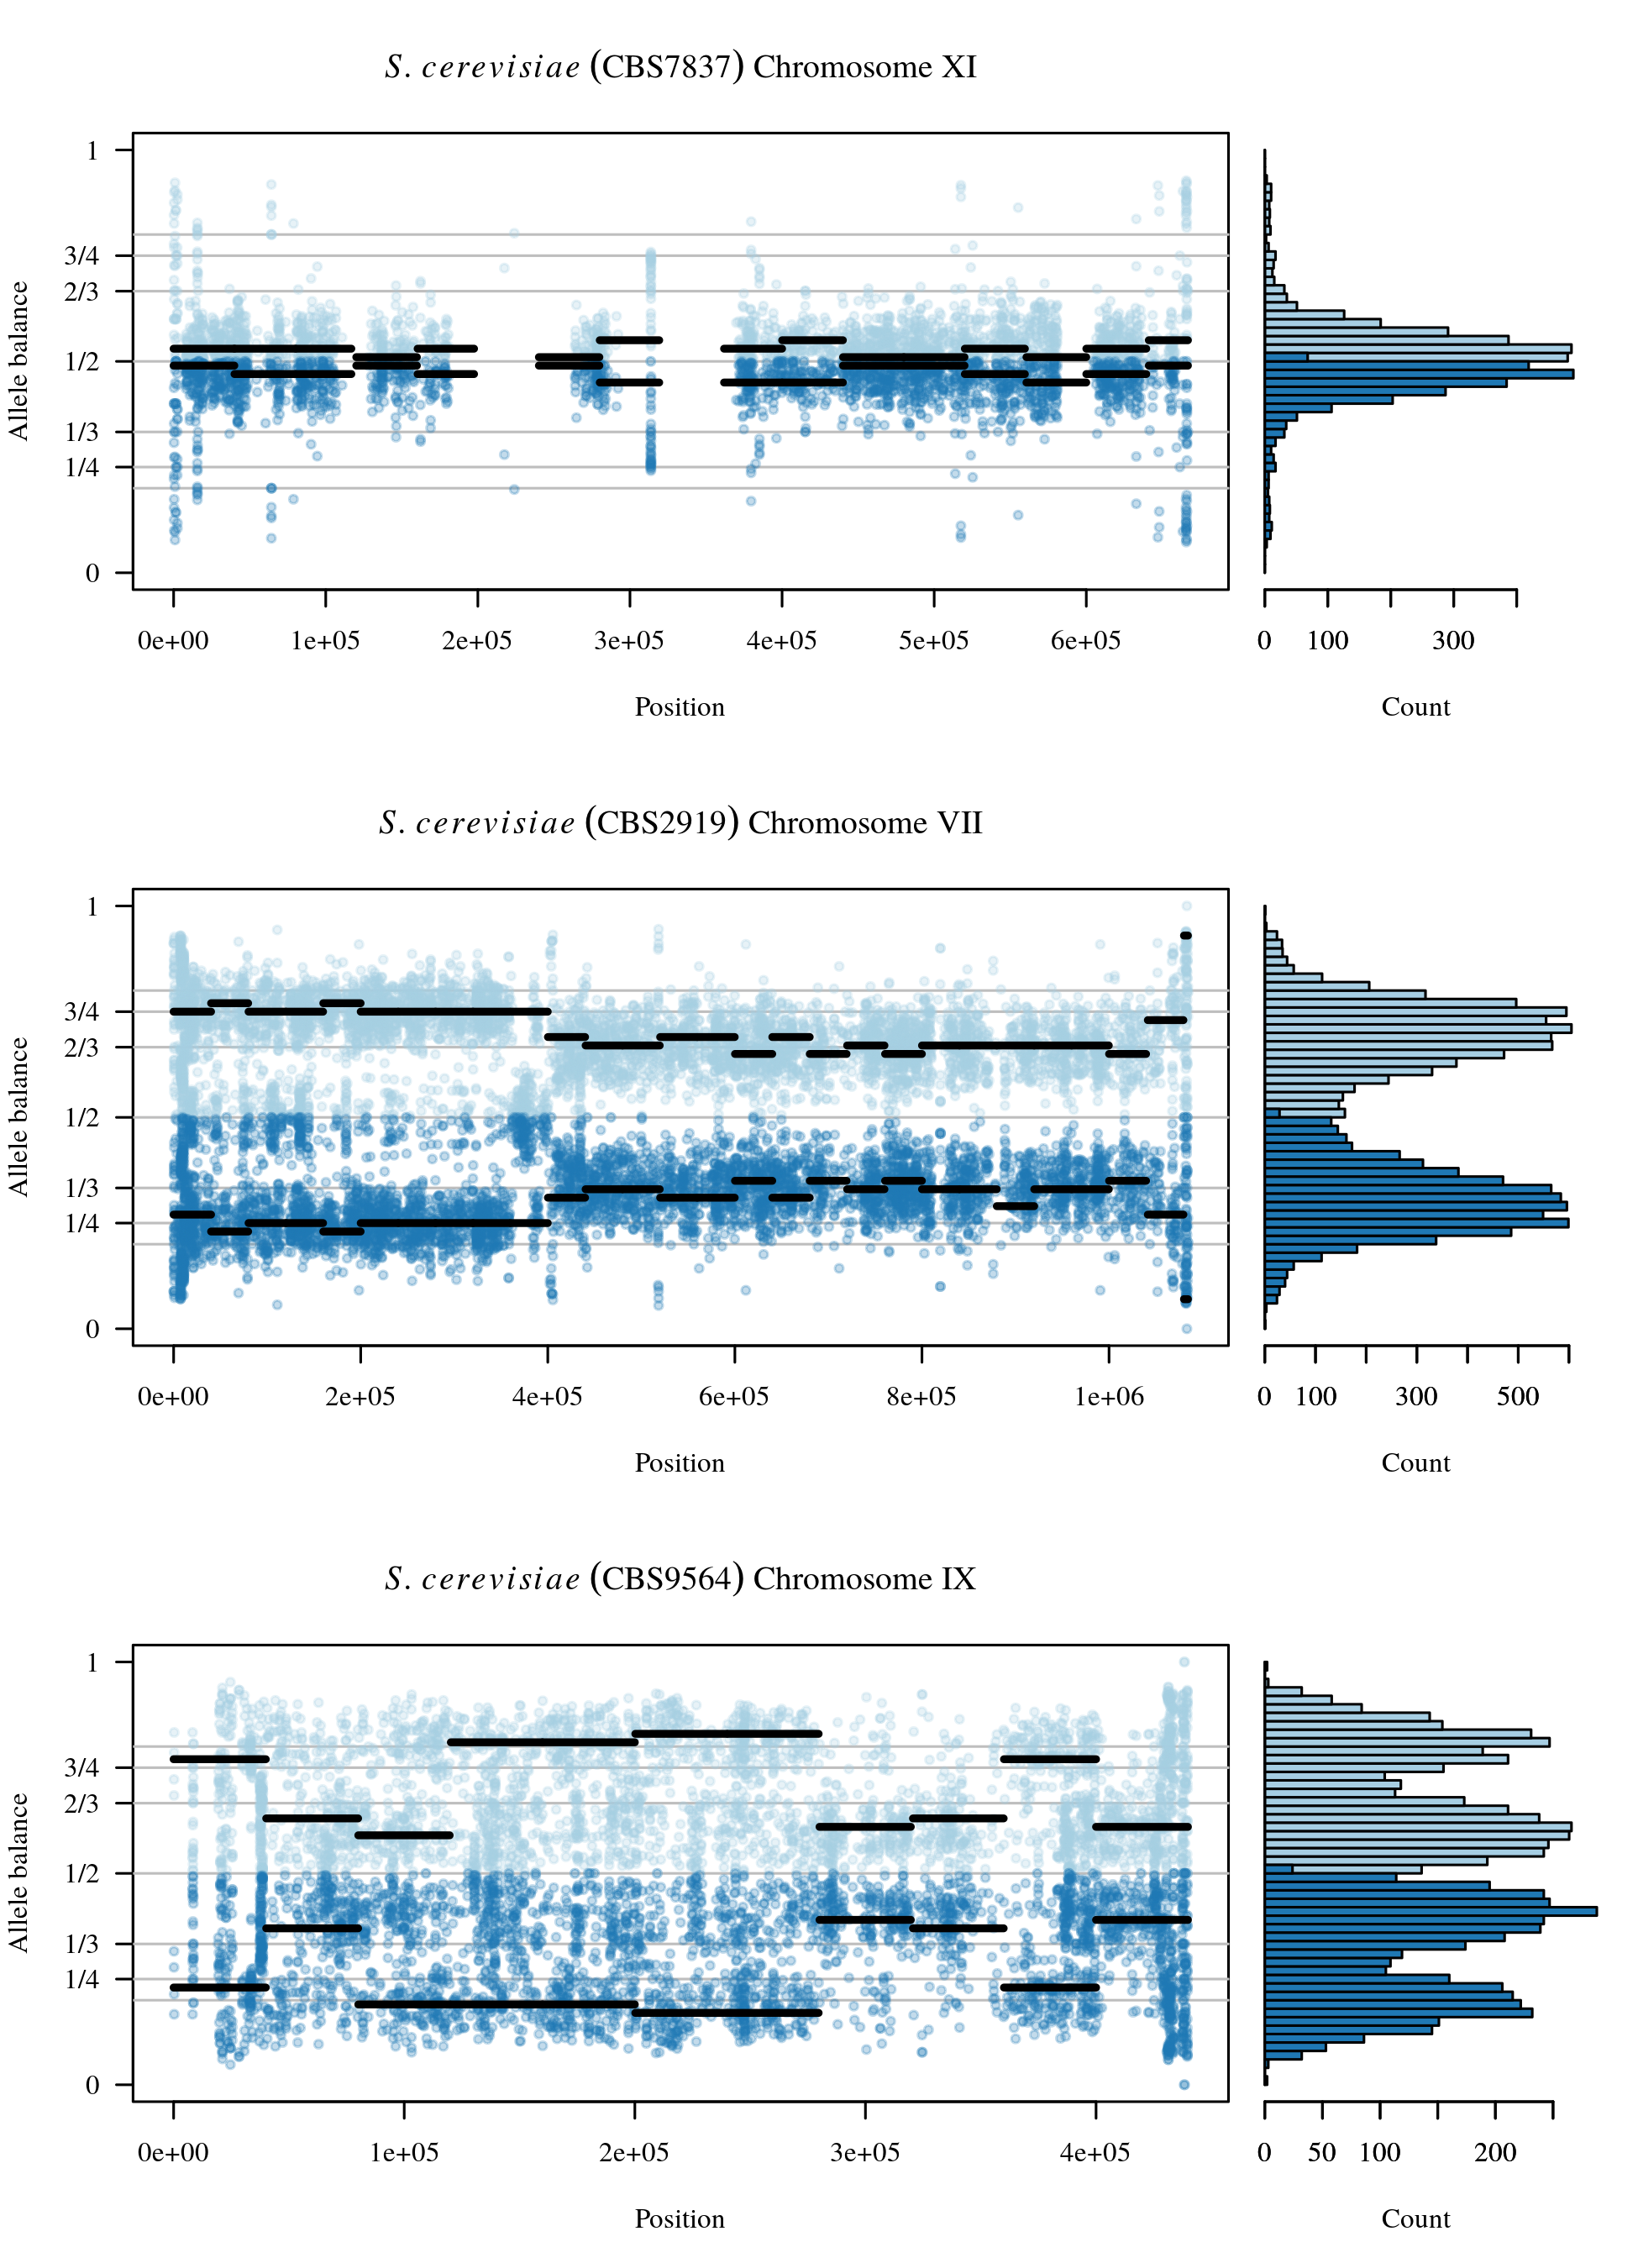
\includegraphics[height=20cm]{./figures/fig6_exemplars.png}
        \end{column}
      \end{columns}

    \end{block}
  \end{column}

  \begin{column}{0.32\textwidth}
    \begin{block}{\large Acknowledgments}
\tiny
\vspace{5mm}

This research is supported in part by U.S. Department of Agriculture (USDA) Agricultural Research Service Grant 5358-22000-039-00D and USDA National Institue of Food and Agriculture Grant 2011-68004-30154.
\newline
\vspace{10mm}

\textit{Saccharomyces cerevisiae} data from:
Zhu YO, Sherlock G, Petrov DA. 
Whole genome analysis of 132 clinical \textit{Saccharomyces cerevisiae} strains reveals extensive ploidy variation.
G3. 2016; 6(8):2421-34. https://doi.org/10.1534/g3.116.029397.
\newline
\vspace{10mm}

vcfR can be found at:
https://CRAN.R-project.org/package=vcfR

\vspace{15mm}

    \end{block}
  \end{column}
\end{columns}




  \end{frame}
\end{document}

